\section{Основні елементарні функції комплексної змінної.}
\subsection{Показникова функція $\exp z$.}
$z\in\Cn,\tab z=xiy\\\\$
$\deff\exp z=e^x(\cos y+isiny)\\\\$
\textbf{Основні властивості}:
\begin{enumerate}
	\item При $z=x\in\Rn$ співпадає з $e^x$.
		\begin{prooff}
			$\exp z|_{z=x}=\exp x=\langle y=0\rangle=e^x$
		\end{prooff}
	\item При $z=iy\>(x=0):\tab \exp iy=e^0(\cos y+i\sin y)=e^{iy}$ - формула Ойлера.
	\item Зберігається властивість: $$\exp z_1\cdot\exp z_2=exp(z_1+z_2)$$ 
		\begin{prooff}
			$\\\exp z_1\cdot\exp z_2=e^{x_1}(\cos y_1+i\sin y_1)\cdot e^{x_2}(\cos y_2+i\sin y_2)=e^{x_1+x_2}\left(\cos(y_1\right.+\\+\left.y_2)+i\sin(y_1+y_2)\right)\eqdef{\exp}=\exp(x_1+x_2+i(y_1+y_2))=\exp(z_1+z_2)$
		\end{prooff}
		\begin{remark*}
			$\exp z=\exp(x+iy)=\exp z\cdot\exp iy=e^x\cdot e^{iy}=e^x(\cos y+isiny)$
		\end{remark*}
	\item $\forall z\tab\exp z\neq0$.
		\begin{prooff}
			$\\$Відомо, що $W=0\Longleftrightarrow|W|=0.\tab |\exp z|=|e^x(\cos y+isiny)|=|e^x|\cdot\\\cdot\underbrace{|\cos y+isiny|}_{|e^{i\varphi}|}=|e^x|\cdot\sqrt{\cos^ y+\sin^2y}=e^x>0\tab\forall z\in\Cn.$
		\end{prooff}
	\item Періодична $T=2\pi i$.
		\begin{prooff}$ $
			\begin{enumerate}
				\item Нехай $W=\exp z$. \\Тоді для $z+2\pi ik:\tab\exp(z+2\pi ik)=\exp(z+i(y+2\pi k))=e^x(\cos(y+\xcancel{2\pi k})+i\sin(y+\xcancel{2\pi k}))=\exp z=W$
				\item Нехай $W=\exp z_1$ і $W=\exp z_2$.\\ $e^{x_1}(\cos y_1+i\sin y_1)=e^{x_2}(\cos y_2+i\sin y_2)\Longrightarrow\begin{cases}
					e^{x_1}=e^{x_2}\\y_2=y_1+2\pi k,\tab k\in\Zn
				\end{cases}\\\Longrightarrow x_1=x_2$. Тоді $z_2-z_1=x_2+iy_2-(x_1+iy_1)=x_1+i(y_1+2\pi k)-(x_1+iy_1)=2\pi ik$
			\end{enumerate}
		\end{prooff}
\end{enumerate}
\subsection{Логарифмічна функція $\Ln z$.}
$z\in\Cn,\tab(z=x+iy)\\\\$
$\deff W=\Ln z,$ якщо $\exp W=z$
\textbf{Основні властивості}:
\begin{enumerate}
	\item $\Ln z$ - багатозначна, бо $\exp$ - періодична функція.
	\item Визначена на $\forall z\in\Cn\backslash\{0\}$ ($\exp$ не може перетворюватись на 0).
	\item При $z=x\in\Rn$ співпадає з $\Ln x$ (тому що $e^x$ буде обереною функцією).
	\item Зберігається властивість: $$\Ln(z_1\cdot z_2)=\Ln z_1+\Ln z_2$$
		\begin{prooff}
			$\\$Нехай $W_1=\Ln z_1,\>W_2=\Ln z_2\Longleftrightarrow z_1=\exp W_1,\>z_2=\exp W_2$. Знайдемо $z_1\cdot z_2:\tab z_1\cdot z_2=\exp W_1\cdot\exp W_2=\exp(W_1+W_2)$. Тоді $\Ln(z_1\cdot z_2)=W_1+W_2=\Ln z_1+\Ln z_2$.
		\end{prooff}
	\item Усі значення $\Ln z:$ $$\Ln z=\ln|z|+i\Arg z$$
		\begin{prooff}
			$\Ln z=\langle z=|z|(\cos(\arg z+2\pi k)+i\sin(\arg z+2\pi k))\rangle=\Ln(|z|\exp(i\Arg z)=\\=\Ln|z|+\Ln(\exp(\Arg z))=\langle|z|\in\Rn,\>|z|>0,\>z\neq 0\Rightarrow \Ln|z|=\ln|z|\rangle=\ln|z|+i\Arg z$
		\end{prooff}
	\item 
\end{enumerate}
\subsection{Тригонометричні функції.}
$z\in\Cn,\tab(z=x+iy)\\\\$
$\deff \sin z=\dfrac1{2i}(\exp(iz)-\exp(-iz))\\\\\tab\tab\tab\tab\>\cos z=\dfrac12(\exp(iz)-\exp(-iz))\\\\\tab\tab\tab\tab\>\tan z=\dfrac{\sin z}{\cos z},\tab \cot z=\dfrac{\cos z}{\sin z}\\\\$
\textbf{Основні властивості}:
\begin{enumerate}
	\item Визначені на $\forall z\in\Cn:$ $$\sin(-z)=-\sin z,\tab \cos(-z)=\cos z$$
	\item При $z=x\in\Rn$ співпадає з $\sin x,\>\cos x$.
		\begin{prooff}
			$\\\sin z|_{z=x}=\dfrac1{2i}(\exp(ix)-\exp(-ix))=\dfrac1{2i}(\cos x+i\sin x-(cos x-i\sin x))=\sin x$. Аналогічно з $\cos z|_{z=x}=\cos x$. 
		\end{prooff}
	\item ($\exp z$ - період $T=2\pi i\Longrightarrow\exp iz :T=2\pi$) $$T_{\sin z,\cos z}=2\pi,\tab T_{\tan z,\cot z}=\pi$$
	\item Зберігаються усі тригинометричні формули. Зокрема:
		$$\sin(z_1+z_2)=\sin z_1\cos z_2+\cos z_1\sin z_2$$
		$$\cos(z_1+z_2)=\cos z_1\cos z_2+\sin z_1\sin z_2$$
		\begin{prooff}
			\begin{align*}
				\deff \sin z,\>\cos z\tab\Longrightarrow\tab & \textrm{1) }\exp iz=\cos z+i\sin z \tag{$\ast$}\\
				&\textrm{2) }\exp(-iz)=\cos z-i\sin z \tag{$\ast\ast$}
			\end{align*}
			При $z=z_1+z_2:\\$
			\begin{enumerate}[label=\arabic*)]
				\item $\exp i(z_1+z_2)\equset{\textrm{в-сть }exp}\exp iz_1\cdot\exp iz_2\equset{(\ast)}(\cos z_1+i\sin z_1)(\cos z_2+i\sin z_2)=\\=\cos z_1\cdot\cos z_2-\sin z_1\cdot\sin z_2+i(\sin z_1\cdot\cos z_2+\cos z_2\cdot\sin z_2)$
				\item $\exp(-i(z_1+z_2))=\exp(-iz_1)\cdot\exp(-iz_2)=(\cos z_1+i\sin z_1)(\cos z_2+i\sin z_2)=\\=\cos z_1\cdot\cos z_2-\sin z_1\cdot\sin z_2-i(\sin z_1\cdot\cos z_2+\cos z_2\cdot\sin z_2)$
			\end{enumerate}
			$\\\dfrac{(1)+(2)}{2}:\tab \cos z_1\cdot\cos z_2-\sin z_1\cdot \sin z_2=\dfrac12(\exp i(z_1+z_2)+\exp(-i(z_1+z_2))\eqdef{}\\=\cos(z_1+z_2)\\\\\dfrac{(1)-(2)}{2}:\tab\sin z_1\cdot \cos z_2+\cos z_1\cdot\sin z_2=\dfrac1{2i}(\exp i(z_1+z_2)-\exp(-(z_1+z_2))\eqdef{}\\=\sin(z_1+z_2)$
		\end{prooff}
		Надаючи $z_1$ та $z_2$ різні значення, можжна отримати усі інші тригонометричні формули. При $z=z_1=z_2:\tab \sin z\cdot\cos z+\cos z\cdot\sin z=2\sin z\cdot\cos z=\sin 2z$. При $z_1=z,z_2=-z:\cos z\cdot\cos(-z)-\sin z\cdot\sin(-z)=\cos^2z+\sin^2z=1=\cos 0$. При $z_1=\dfrac\pi2,z_2=z:\sin\dfrac\pi2\cdot\cos z+\cos\dfrac\pi2\cdot\sin z=\cos z=\sin\left(\dfrac\pi2+z\right)$
	\item \begin{align*}
		\sin z=0\tab\Longleftrightarrow\tab&z=\pi n,\tab n\in\Zn\\
		\cos z=0\tab\Longleftrightarrow\tab&z=\dfrac\pi2+\pi n,\tab n\in\Zn
	\end{align*}
	\begin{prooff}$\>$
		\begin{enumerate}[label=\arabic*)]
			\item $\sin z=0\tab \Longleftrightarrow\tab\dfrac1{2i}(\exp(iz)-\exp(-iz))=0\tab \Longleftrightarrow\tab\exp i(x+iy)=\\=\exp(-i(x+iy).\tab\exp(-y+ix)=\exp(y-ix).\tab \Longleftrightarrow\tab e^{-y}=\\=(\cos x+i\sin x)=e^y(\cos(-x)+i\sin(-x))\tab \Longleftrightarrow\tab$ "=" в триг формі. $\begin{cases}
				e^{-y}=e^y\\ x=-x+2\pi n,\tab n\in\Zn
			\end{cases},
			\begin{cases}
				y=0\\x\pi n,\tab n\in\Zn 
			\end{cases},$ $\\z=x+iy=\pi n,\tab n\in\Zn$
			\item $\cos z=\sin\left(\dfrac\pi2+z\right)=0$
				$\dfrac\pi2+z=\pi k,\tab k\in\Zn,\tab z=-\dfrac\pi2+\pi k=\\=\pi-\dfrac\pi2+\pi(k-1)=\dfrac\pi2+\pi n,\tab n\in\Zn$
		\end{enumerate}
	\end{prooff}
	\item $\sin z,\>\cos z$ не обмежені.\\
		Наприклад для $z=\dfrac\pi2+iy,\tab y\in\Rn:\tab \sin z=\sin\left(\dfrac\pi2+iy\right)=\dfrac1{2i}\left(\exp\left(i\left(\dfrac\pi2+iy\right)\right)\right.-\\-\left.\exp\left(-i\left(\dfrac\pi2+iy\right)\right)\right)=\dfrac1{2i}\left(\exp\left(i\dfrac\pi2-y\right)-\exp\left(y-i\dfrac\pi2\right)\right)=\dfrac1{2i}\left(e^{-y}\left(\cos\dfrac\pi2+i\sin\dfrac\pi2\right)\right.-\\-\left.e^{-y}\left(\cos\dfrac\pi2-i\sin\dfrac\pi2\right)\right)=\dfrac12\left(e^{-y}+e^{y}\right).$
\end{enumerate}
\subsection{Гіперболічні функції.}
$z=x+iy,\tab x,y\in\Rn\\\\$
$\deff\sh z=\dfrac12(\exp z-\exp(-z))\\\tab\tab\tab\tab\>\ch z=\dfrac12(\exp z+\exp(-z)\\\tab\tab\tab\tab\>\th z=\dfrac{\sh z}{\ch z}\\\tab\tab\tab\tab\>\cth z=\dfrac{\ch z}{\sh z}\\\\$
\textbf{Основні властивості}:
\begin{enumerate}
	\item Визначені на $\forall z\in\Cn:$ $$\sh(-z)=-\sh(z),\tab\ch(-z)=\ch(z)$$
	\item При $z=x\in\Rn$ співпадає з $\sh x,\ch x$
		\begin{prooff}
			В цьому випадку $\exp x= e^x$, і звідци це встановлюється.
		\end{prooff}
	\item Періодичні: $$T_{\sh,\ch}=2\pi i,\tab T_{\th,\cth}=\pi i$$
	\item Зв'язок з тригонометричними функціями: $$\sin iz=i\sh z,\tab \cos iz=i\ch z$$
\end{enumerate}
Обернені тригонометричні і гіперболічні функції:\\\\ $\deff W=\arcsin z,\tab \sin W=z$
\subsection{Степінь з комплексним показником. Загальна степенева $(z^\alpha)$ та показникова $\alpha^z$ функції}
Нехай $\alpha,\beta\in\Cn,\tab\alpha^\beta$ - множина значень. В загальному випадку $\alpha^{\beta_1}\cdot\alpha^{\beta_2}\neq\alpha^{\beta_1+\beta_2}.\\\\$
$\deff\alpha^\beta=\exp(\beta\Ln\alpha)\\\\$
Загальна степенева функція: 
$\\\\\deff f(z)=z^\alpha=\exp(\alpha\Ln z),\tab\alpha\in\Cn\\$
$z^\alpha=\exp(\alpha\Ln z)=\langle\alpha=a+ib,\tab a,b\in\Rn,\tab z=|z|\cdot e^{i\varphi}\rangle=\exp((a+ib)(\ln|z|+\\+i(\varphi+2\pi k)))=\exp(a\ln|z|-b(\varphi+2\pi k)+i(a(\varphi+2\pi k)+b\ln|z|))=e^{a\ln|z|-b(\varphi+2\pi k)}\cdot\\\cdot(\cos(a(\varphi+2\pi k)+b\ln|z|)+i\sin(a(\varphi+2\pi k)+b\ln|z|))\\\\$
При $\alpha\in\Rn:$
\begin{itemize}
	\item[-]  якщо $\alpha=n\in\Zn\>(a=n\in\Zn,b=0):\\z^\alpha|_{\alpha=n}=e^{n\ln|z|}\cdot(\cos(n(\varphi+2\pi k)))+i\sin(n(\varphi+2\pi k))=e^{n\ln|z|}\cdot(\cos n\varphi+i\sin n\varphi)=\\=|z|^n,\tab n\in\Zn$
	\item[-]  якщо $\alpha=\dfrac1n\in\Rn\>\left(a=\dfrac1n\in\Zn,b=0\right):\\z^\alpha|_{\alpha=\frac1n}=e^{\frac1n\ln|z|}\cdot\left(\cos\left(\dfrac1n\varphi+2\pi k)\right)+i\sin\left(\dfrac1n(\varphi+2\pi k)\right)\right)=|z|^\frac1n\left(\cos\dfrac{\varphi+2\pi k}{n}\right.+\\+\left.i\sin\dfrac{\varphi+2\pi k}{n}\right)=\sqrt[n]{z}$
\end{itemize}
Загальна показникова функція: 
$\\\\\deff f(z)=\alpha^z=\exp(z\Ln \alpha),\tab a\in C\\\\$
$\alpha^z=\exp(z\Ln \alpha)=\langle z=x+iy,\tab x,y\in\Rn,\tab\alpha=|z|e^{i\psi}\rangle=\exp((x+iy)(\ln|\alpha|+\\+i(\psi+2\pi k)))=\exp(x\ln|\alpha|-u(\psi+2\pi k)+i(y\ln|\alpha|+x(\psi+2\pi k)))=e^{x\ln|\alpha|-y(\psi+2\pi k)}\cdot\\\cdot(\cos(y\ln|\alpha|+x(\psi+2\pi k))+i\sin(y\ln|\alpha|+x(\psi+2\pi k)))\\\\$
При $\alpha\in\Rn:\tab (|e|=e,\psi=0)$
\begin{itemize}
	\item[-]  $e^z=e^{x\ln e-y\cdot2\pi k}\cdot(\cos(y\ln e+x\cdot2\pi k)+i\sin(y\ln e+x\cdot2\pi k))$
	\item[-] При $k=0:\tab e^z|_{k=0}=e^{x}\cdot(\cos y+i\sin y)=\exp z$
\end{itemize}
\section{Границя функції. Неперервність.}
Нехай $z=x+iy,\tab z_0=x_0+iy_0,\tab A\in\Cn\\\\\deff\lim\limits_{z\to z_0}f(z)=A,$ якщо $\forall\varepsilon>0\>\>\>\>\exists\delta(\varepsilon)>0\>\>\>\>(0<|z-z_0|<\delta(\varepsilon))\Rightarrow|f(z)-A|<\varepsilon)$
\begin{figure*}[htp]\centering
	\begin{tikzpicture}
		\begin{axis}[ticks=none,axis lines=middle, xmin=-0.1, xmax=0.9,ymin=-0.1,ymax=0.9,xshift=-3.4cm]	
		\end{axis}
		\draw (0,0) node {\small$z=x+iy$};
		\draw (-2.5,5.5) node {$y$};
		\draw (3,1) node {$x$};
		\draw (0,3) node[circle,fill,inner sep=1pt] {};
		\draw (0,3) node[below] {\scriptsize$z_0$};
		\draw (0,3) -- (1.06,4.06) node[sloped,midway,above] {\scriptsize$z$};
		\draw (1.06,4.06) node[right] {\scriptsize$\delta(\varepsilon)$};
		\draw[->] (3,3.5) -- (4,3.5) node[midway,above] {$f$};
		\draw (0,3) circle (1.5);
 	    \clip (0,3) circle (1.5);
 		\pgfmathsetseed{24122015}
    	\foreach \p in {1,...,300}
    	{ \pgfmathsetmacro{\x}{2*rand}
        	\pgfmathsetmacro{\y}{rand*sqrt(4-pow(\x,2))+3}
        	\fill[black]    (\x,\y) circle (0.02);
    	}
	\end{tikzpicture}
	\begin{tikzpicture}
		\begin{axis}[ticks=none,axis lines=middle, xmin=-0.1, xmax=0.9,ymin=-0.1,ymax=0.9,xshift=-3.4cm]	
		\end{axis}
		\draw (0,0) node {\small$f(z)=u+iv$};
		\draw (-2.5,5.5) node {$v$};
		\draw (3,1) node {$u$};
		\draw (0,3) node[circle,fill,inner sep=1pt] {};
		\draw (0,3) node[above] {\scriptsize$A$};
		\draw (0,3) -- (1.06,1.95) node[sloped,midway,above] {\scriptsize$\varepsilon$};
		\draw (1.06,1.95) node[right] {\scriptsize$f(z)$};
		\draw (0,3) circle (1.5);
 	    \clip (0,3) circle (1.5);
 		\pgfmathsetseed{24122015}
    	\foreach \p in {1,...,300}
    	{ \pgfmathsetmacro{\x}{2*rand}
        	\pgfmathsetmacro{\y}{rand*sqrt(4-pow(\x,2))+3}
        	\fill[black]    (\x,\y) circle (0.02);
    	}
	\end{tikzpicture}
\end{figure*}
$\\\lim\limits_{z\to z_0}f(z)=\left\langle\begin{array}{c}
	f(z)=u(x,y)+iv(x,y)\\z=x+iy
\end{array} \right\rangle=\lim\limits_{\scriptsize\begin{array}{c}
	x\to x_0\\y\to y_0
\end{array}}(u+iv).\\ f\to A,g\to B$ при $z\to z_0.\tab $ Тоді 
\begin{align*}
	\tab\lim\limits_{z\to z_0}(f+g)=&\lim\limits_{z\to z_0}f+\lim\limits_{z\to z_0}g\\\lim\limits_{z\to z_0}(f\cdot g)=&\lim\limits_{z\to z_0}f\cdot\lim\limits_{z\to z_0}g\\\lim\limits_{z\to z_0}\left(\dfrac fg\right)=&\dfrac{\lim\limits_{z\to z_0}f}{\lim\limits_{z\to z_0}g},\tab \lim\limits_{z\to z_0}g\neq0
\end{align*}
$\\\deff\lim\limits_{z\to z_0} f(z)=\infty,$ якщо $\forall\varepsilon>0\tab\exists\delta(\varepsilon)>0\tab(0<|z-z_0|<\delta(\varepsilon)\Rightarrow|f(z)|>\varepsilon)\\$
\begin{figure*}[htp]\centering
	\begin{tikzpicture}
		\begin{axis}[ticks=none,axis lines=middle, xmin=-0.1, xmax=0.9,ymin=-0.1,ymax=0.9,xshift=-3.4cm]	
		\end{axis}
		\draw (-2.5,5.5) node {$y$};
		\draw (3,1) node {$x$};
		\draw (0,3) node[circle,fill,inner sep=1pt] {};
		\draw (0,3) node[below] {\scriptsize$z_0$};
		\draw (0,3) -- (1.06,4.06) node[sloped,midway,above] {\scriptsize$z$};
		\draw[->] (3,3.5) -- (4,3.5) node[midway,above] {$f$};
		\draw (0,3) circle (1.5);
 	    \clip (0,3) circle (1.5);
 		\pgfmathsetseed{24122015}
    	\foreach \p in {1,...,300}
    	{ \pgfmathsetmacro{\x}{2*rand}
        	\pgfmathsetmacro{\y}{rand*sqrt(4-pow(\x,2))+3}
        	\fill[black]    (\x,\y) circle (0.02);
    	}
	\end{tikzpicture}
	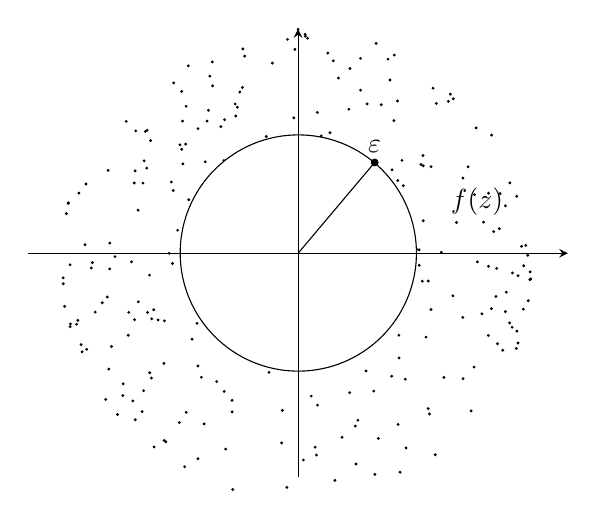
\begin{tikzpicture}
		\pgfmathsetseed{24122015}
    	\foreach \p in {1,...,300}
    	{ \pgfmathsetmacro{\x}{3*rand}
        	\pgfmathsetmacro{\y}{rand*sqrt(9-pow(\x,2))+2.7}
        	\fill[black]    (\x,\y) circle (0.02);
    	}
    	\draw[fill=white] (0.03,2.85) circle (1.5);
		\begin{axis}[ticks=none,axis lines=middle, xmin=-0.5, xmax=0.5,ymin=-0.5,ymax=0.5,xshift=-3.4cm]	
		\end{axis}
		\draw (1,4) node[circle,fill,inner sep=1pt] {};
		\draw (0.03,2.85) -- (1,4) node[right,above] {$\varepsilon$};
		\draw (2.3,3.5) node {$f(z)$};
	\end{tikzpicture}
\end{figure*}

























